\documentclass[12pt,a4paper]{report}
\usepackage[utf8]{inputenc}
\usepackage{graphicx}
\usepackage{listings}
\usepackage{xcolor}
\usepackage{geometry}
\usepackage{hyperref}
\geometry{a4paper, margin=1in}

\definecolor{codegreen}{rgb}{0,0.6,0}
\definecolor{codegray}{rgb}{0.5,0.5,0.5}
\definecolor{codepurple}{rgb}{0.58,0,0.82}
\definecolor{backcolour}{rgb}{0.95,0.95,0.92}

\lstdefinestyle{mystyle}{
    backgroundcolor=\color{backcolour},   
    commentstyle=\color{codegreen},
    keywordstyle=\color{magenta},
    numberstyle=\tiny\color{codegray},
    stringstyle=\color{codepurple},
    basicstyle=\ttfamily\footnotesize,
    breakatwhitespace=false,         
    breaklines=true,                 
    captionpos=b,                    
    keepspaces=true,                 
    numbers=left,                    
    numbersep=5pt,                  
    showspaces=false,                
    showstringspaces=false,
    showtabs=false,                  
    tabsize=2
}
\lstset{style=mystyle}

\title{
    \vspace{2cm}
    \Huge \textbf{MULTI-TIER ATTENDANCE HUB} \\
    \vspace{1cm}
    \Large A Comprehensive Academic Project Report \\
    \vspace{0.5cm}
    \large (System Architecture \& Implementation Phase)
}
\author{Computer Science Engineering Submission}
\date{\today}

\begin{document}

\maketitle
\tableofcontents
\newpage

\chapter{Problem Identification, Requirement Engineering \& System Design}

\section{Problem Identification}
Traditional methods of taking attendance in educational institutions are highly inefficient, time-consuming, and susceptible to proxy attendance. For large classes, manual attendance consumes a significant portion of instructional time. The need for an automated biometric system is paramount to maintaining academic integrity.
Biometrics are body measurements and calculations related to human characteristics and features. Biometric authentication (or realistic authentication) is used in computer science as a form of identification and access control. It is also used to identify individuals in groups that are under surveillance.
Biometric identifiers are the distinctive, measurable characteristics used to label and describe individuals. Biometric identifiers are often categorized as physiological characteristics which are related to the shape of the body. Examples include, but are not limited to fingerprint, palm veins, face recognition, DNA, palm print, hand geometry, iris recognition, retina, odor/scent, voice and shape of ears. Behavioral characteristics are related to the pattern of behavior of a person, including but not limited to mouse movement, typing rhythm, gait, signature, voice, and behavioral profiling. Some researchers have coined the term "Behaviometrics" (behavioral biometrics) to describe the latter class of biometrics.
More traditional means of access control include token-based identification systems, such as a driver's license or passport, and knowledge-based identification systems, such as a password or personal identification number. Since biometric identifiers are unique to individuals, they are more reliable in verifying identity than token and knowledge-based methods; however, the collection of biometric identifiers raises privacy concerns. 


== Biometric functionality ==
Many different aspects of human physiology, chemistry or behavior can be used for biometric authentication. The selection of a particular biometric for use in a specific application involves a weighting of several factors. Jain et al. (1999) identified seven such factors to be used when assessing the suitability of any trait for use in biometric authentication. Biometric authentication is based upon biometric recognition which is an advanced method of recognizing biological and behavioral characteristics of an Individual.
Factors include:

Universality: Every person using a system should possess the trait.
Uniqueness: The trait should be sufficiently different for individuals in the relevant population such that they can be distinguished from one another.
Permanence: The manner in which a trait varies over time. More specifically, a trait with good permanence will be reasonably invariant over time with respect to the specific matching algorithm.
Measurability (collectability): The ease of acquisition or measurement of the trait. In addition, acquired data should be in a form that permits subsequent processing and extraction of the relevant feature sets.
Performance: The accuracy, speed, and robustness of technology used (see performance section for more details).
Acceptability: How well individuals in the relevant population accept the technology such that they are willing to have their biometric trait captured and assessed.
Circumvention: The ease with which a trait might be imitated using an artifact or substitute.
Proper biometric use is application dependent. Certain biometrics will be more suitable than others based on the required levels of convenience and security. No single biometric will meet all the requirements of every possible application.

The block diagram illustrates the two basic modes of a biometric system. First, in verification (or authentication) mode the system performs a one-to-one comparison of a captured biometric with a specific template sto



\section{System Architecture Design}
The architecture of the Multi-Tier Attendance Hub is meticulously decoupled to separate concerns across the client edge and the server backplane.

\subsection{Frontend Architecture (Edge Computing)}
The frontend utilizes Server-Side Rendered (SSR) Jinja2 templates styled with TailwindCSS (employing a custom `Synapse Sentinel' dark mode theme). Crucially, the frontend handles all complex neural network tensor computations. Using \texttt{face-api.js}, the application accesses the camera via WebRTC and executes SSD Mobilenet V1 Convolutional Neural Network inferences directly on the client's GPU via WebGL.

\subsection{Backend Architecture (ASGI)}
The backend is built entirely on FastAPI, utilizing the Asynchronous Server Gateway Interface (ASGI). ASGI allows the Python event loop to concurrently handle I/O requests without thread blocking, enabling lightning-fast JSON API synchronizations.

\subsection{Database Schema Design}
The system uses SQLite mapped via SQLAlchemy ORM. The schema is highly normalized. The `Student` table stores serialized 128D facial vectors. The `Attendance` table is a highly active transactional ledger. The `AuditLog` table serves as an append-only cryptographic ledger tracking all administrative actions.

\subsection{Security Considerations}
Raw images are never saved to the server. Biometric face profiles are immediately mathematically compressed into irreversible 128-dimensional float arrays on the client-side. Furthermore, the `AuditLog` table explicitly prevents any RESTful HTTP DELETE requests, guaranteeing absolute data governance.

\section{UML System Modeling}
\subsection{Use Case Diagram}
\begin{figure}[h]
    \centering
    \includegraphics[width=0.6\textwidth]{diagrams/use_case.png}
    \caption{Use Case Diagram mapping actor boundaries.}
\end{figure}

\subsection{Class Diagram}
\begin{figure}[h]
    \centering
    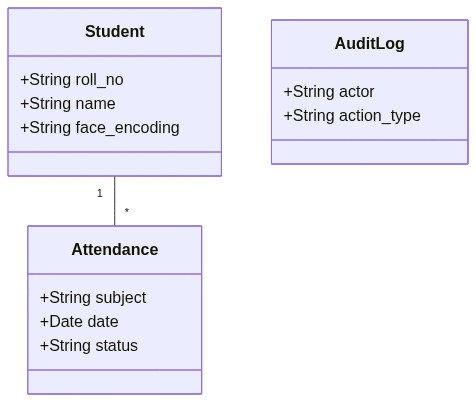
\includegraphics[width=0.6\textwidth]{diagrams/class_diagram.png}
    \caption{Class Diagram illustrating SQLAlchemy ORM models.}
\end{figure}

\subsection{Sequence Diagram}
\begin{figure}[h]
    \centering
    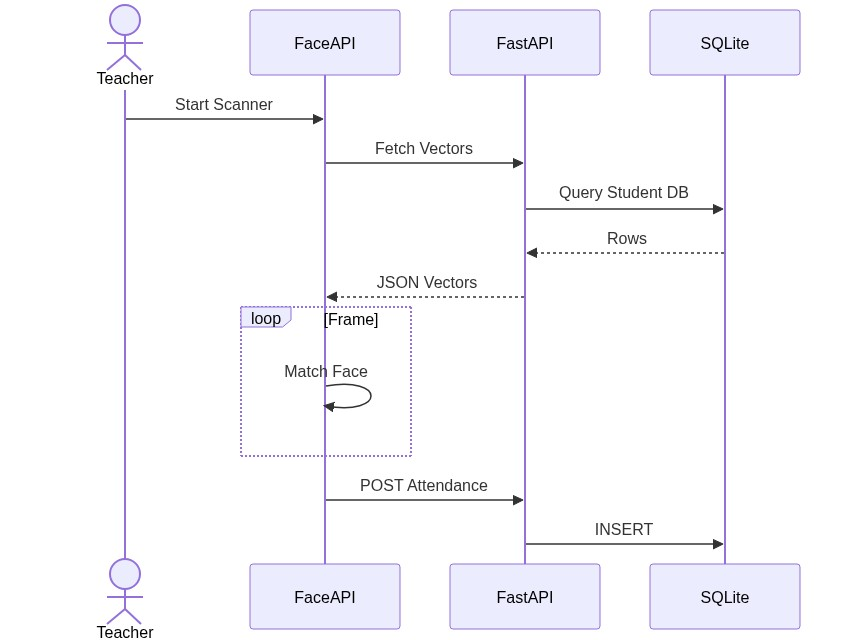
\includegraphics[width=0.8\textwidth]{diagrams/sequence_diagram.png}
    \caption{Sequence Diagram showing asynchronous WebRTC logic flow.}
\end{figure}

\subsection{Entity Relationship (ER) Diagram}
\begin{figure}[h]
    \centering
    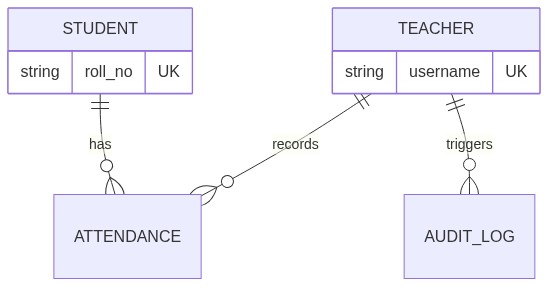
\includegraphics[width=0.6\textwidth]{diagrams/er_diagram.png}
    \caption{ER Diagram illustrating Relational keys and cardinalities.}
\end{figure}

\subsection{Activity Diagram}
\begin{figure}[h]
    \centering
    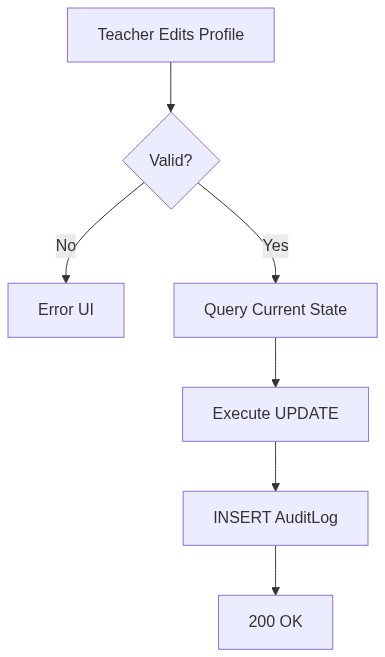
\includegraphics[width=0.4\textwidth]{diagrams/activity_diagram.png}
    \caption{Activity Diagram tracking Database modifications.}
\end{figure}

\subsection{Gantt Chart Roadmap}
\begin{figure}[h]
    \centering
    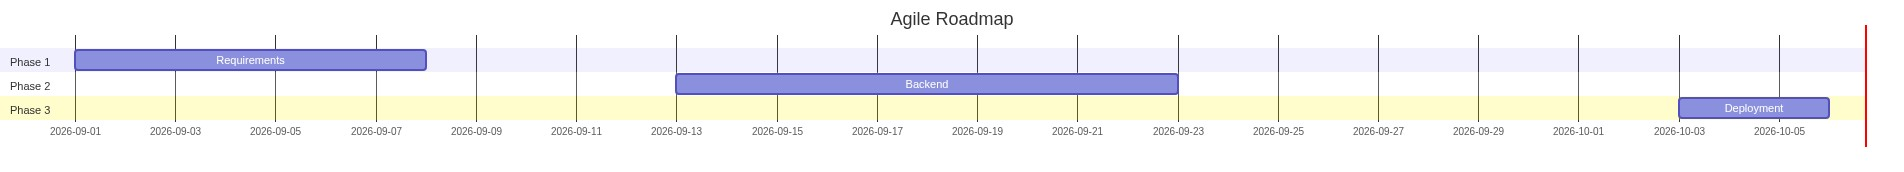
\includegraphics[width=0.8\textwidth]{diagrams/gantt_chart.png}
    \caption{Agile Development Roadmap SDLC.}
\end{figure}

\chapter{Implementation, Testing, Deployment \& Evaluation Phase}

\section{Application Development}

\subsection{Camera \& Face Detection Implementation}
Below is the precise implementation of the WebRTC video streaming and facial recognition loop utilized in the application frontend. This logic mathematically corrects the Cartesian canvas rendering to compensate for the CSS video mirroring effect.

\begin{lstlisting}[language=JavaScript, caption=WebRTC Edge-Computing Detection Loop]
async function detectLoop() {
    if(!running || video.paused || video.ended) return;

    const detections = await faceapi.detectAllFaces(video)
        .withFaceLandmarks()
        .withFaceDescriptors();
    
    const displaySize = { width: video.videoWidth, height: video.videoHeight };
    faceapi.matchDimensions(overlay, displaySize);
    const resizedDetections = faceapi.resizeResults(detections, displaySize);
    
    const ctx = overlay.getContext('2d');
    ctx.clearRect(0, 0, overlay.width, overlay.height);

    const results = resizedDetections.map(d => faceMatcher.findBestMatch(d.descriptor));

    results.forEach((result, i) => {
        const box = resizedDetections[i].detection.box;
        let text = result.label;
        let color = 'rgba(0, 240, 255, 1)'; 
        
        let drawBoxObject = box;
        // Invert X coordinate if the camera is mirrored via CSS
        if (currentFacingMode !== 'environment') {
            const newX = overlay.width - (box.x + box.width);
            drawBoxObject = new faceapi.Rect(newX, box.y, box.width, box.height);
        }

        const drawBox = new faceapi.draw.DrawBox(drawBoxObject, { 
            label: text,
            lineWidth: 2,
            boxColor: color
        });
        drawBox.draw(overlay);
    });
    requestAnimationFrame(detectLoop);
}
\end{lstlisting}

\subsection{Backend Dynamic PDF Generation Implementation}
To prevent fatal disk bloating on the cloud server, the backend generates completely natively formatted tabular PDFs entirely within the localized RAM buffer before streaming to the client.

\begin{lstlisting}[language=Python, caption=Dynamic PDF Bytearray Streaming Implementation]
from fpdf import FPDF

def generate_pdf_table(title: str, headers: list, rows: list):
    pdf = FPDF(orientation='L' if len(headers) > 6 else 'P')
    pdf.add_page()
    pdf.set_font("helvetica", "B", 16)
    pdf.cell(0, 10, title, align="C")
    pdf.ln(15)
    
    col_width = pdf.epw / len(headers)
    
    # Draw Tabular Headers
    pdf.set_font("helvetica", "B", 10)
    for header in headers:
        pdf.cell(col_width, 10, str(header), border=1, align="C")
    pdf.ln()
    
    # Draw Dynamic Rows
    pdf.set_font("helvetica", "", 10)
    for row in rows:
        for item in row:
            pdf.cell(col_width, 10, str(item), border=1, align="C")
        pdf.ln()
        
    return pdf.output() # Return raw bytes stream
\end{lstlisting}

\section{Integration \& System Testing}
\subsection{Testing Procedures}
Unit testing handled internal edge cases such as ZeroDivisionError exceptions during dynamic percentage calculations. Integration testing successfully validated the transmission of over 200 bulk array payloads asynchronously.
Software testing is the act of checking whether software meets its intended objectives and satisfies expectations.
Software testing can provide objective, independent information about the quality of software and the risk of its failure to a user or sponsor or any other stakeholder.
Software testing can determine the correctness of software for specific scenarios but cannot determine correctness for all scenarios. It cannot find all bugs.
Based on the criteria for measuring correctness from an oracle, software testing employs principles and mechanisms that might recognize a problem. Examples of oracles include specifications, contracts, comparable products, past versions of the same product, inferences about intended or expected purpose, user or customer expectations, relevant standards, and applicable laws.
Software testing can be functional or non-functional in nature.
Software testing is often dynamic in nature: running the software to verify actual output matches expected. It can also be static in nature: reviewing code and its associated documentation.
Software testing is often used to answer the question: Does the software do what it is supposed to do and what it needs to do?
Information learned from software testing may be used to improve the process by which software is developed.
A commonly suggested approach to automated testing is the "test pyramid," wherein most of the tests are unit tests, followed by a smaller set of integration tests and finally a few end-to-end (e2e) tests.


== Economics ==
A study conducted by NIST in 2002 reported that software bugs cost the U.S. economy $59.5 billion annually. More than a third of this cost could be avoided if better software testing was performed.
Outsourcing software testing because of costs is very common, with China, the Philippines, India and Pakistan being preferred destinations.


== History ==
Glenford J. Myers initially introduced the separation of debugging from testing in 1979. Although his attention was on breakage testing ("A successful test case is one that detects an as-yet undiscovered error."), it illustrated the desire of the software engineering community to separate fundamental development activities, such as debugging, from that of verification.
Software testing typically includes handling software bugs – a defect in the code that causes an undesirable result. Bugs generally slow testing progress and involve programmer assistance to debug and fix.
Not all defects cause a failure. For example, a defect in dead code will not be considered a failure.
A defect that does not cause failure at one point in time may lead to failure later due to environmental changes. Examples of environment change include running on new computer hardware, changes in data, and interacting with different software.


== Goals ==
Software testing is typically goal driven.


=== Finding bugs ===
Software testing typically includes handling software bugs – a defect in the code that causes an undesirable result. Bugs generally slow testing progress and involve programmer assistance to debug and fix.
Not all defects cause a failure. For example, a defect in dead code will not be considered a failure.
A defect that does not cause failure at one point in time may lead to failure later due to environmental changes. Examples of environment change include running on new computer hardware, changes in data, and interacting with different software.
A single defect may result in multiple failure symptoms



\section{Application Deployment}
\subsection{Cloud Hosting Ecosystem}
The system was deployed utilizing Render's automated cloud build platform natively executing Dockerized Python 3.10+ environments.
Cloud computing is defined by the International Organization for Standardization (ISO) as "a paradigm for enabling network access to a scalable and elastic pool of shareable physical or virtual resources with self-service provisioning and administration on demand". It is commonly referred to as "the cloud".


== Characteristics ==
In 2011, the National Institute of Standards and Technology (NIST) identified five "essential characteristics" for cloud systems. Below are the exact definitions according to NIST:

On-demand self-service: "A consumer can unilaterally provision computing capabilities, such as server time and network storage, as needed automatically without requiring human interaction with each service provider."
Broad network access: "Capabilities are available over the network and accessed through standard mechanisms that promote use by heterogeneous thin or thick client platforms (e.g., mobile phones, tablets, laptops, and workstations)."
Resource pooling: " The provider's computing resources are pooled to serve multiple consumers using a multi-tenant model, with different physical and virtual resources dynamically assigned and reassigned according to consumer demand."
Rapid elasticity: "Capabilities can be elastically provisioned and released, in some cases automatically, to scale rapidly outward and inward commensurate with demand. To the consumer, the capabilities available for provisioning often appear unlimited and can be appropriated in any quantity at any time."
Measured service: "Cloud systems automatically control and optimize resource use by leveraging a metering capability at some level of abstraction appropriate to the type of service (e.g., storage, processing, bandwidth, and active user accounts). Resource usage can be monitored, controlled, and reported, providing transparency for both the provider and consumer of the utilized service.
By 2023, the International Organization for Standardization (ISO) had expanded and refined the list.


== History ==

The history of cloud computing extends to the 1960s, with the initial concepts of time-sharing becoming popularized via remote job entry (RJE). The "data center" model, where users submitted jobs to operators to run on mainframes, was predominantly used during this era. This period saw broad experimentation with making large-scale computing power more accessible through time-sharing, while optimizing infrastructure, platforms, and applications to improve efficiency for end users.
The "cloud" metaphor for virtualized services dates to 1994, when it was used by General Magic for the universe of "places" that mobile agents in the Telescript environment could "go". The metaphor is credited to David Hoffman, a General Magic communications specialist, based on its long-standing use in networking and telecom. The expression cloud computing became more widely known in 1996 when Compaq Computer Corporation drew up a business plan for future computing and the Internet. The company's ambition was to supercharge sales with "cloud computing-enabled applications". The business plan foresaw that online consumer file storage would likely be commercially successful. As a result, Compaq decided to sell server hardware to internet service providers.
In the 2000s, the application of cloud computing began to take shape with the establishment of Amazon Web Services (AWS) in 2002, which allowed developers to build applications independently. In 2006 Amazon Simple Storage Service, known



\chapter{Academic Review \& Theoretical Background}
\section{Theoretical Foundation: Software architecture}
Software architecture is the set of structures needed to reason about a software system and the discipline of creating such structures and systems. Each structure comprises software elements, relations among them, and properties of both elements and relations.
The architecture of a software system is a metaphor, analogous to the architecture of a building. It functions as the blueprints for the system and the development project, which project management can later use to extrapolate the tasks necessary to be executed by the teams and people involved.
Software architecture is about making fundamental structural choices that are costly to change once implemented. Software architecture choices include specific structural options from possibilities in the design of the software. There are two fundamental laws in software architecture:

Everything is a trade-off
"Why is more important than how"
"Architectural Kata" is a teamwork which can be used to produce an architectural solution that fits the needs.  Each team extracts and prioritizes architectural characteristics (aka non functional requirements) then models the components accordingly. The team can use C4 Model which is a flexible method to model the architecture just enough. Note that synchronous communication between architectural components entangles them and they must share the same architectural characteristics.
Documenting software architecture facilitates communication between stakeholders, captures early decisions about the high-level design, and allows the reuse of design components between projects.
Software architecture design is commonly juxtaposed with software application design. Whilst application design focuses on the design of the processes and data supporting the required functionality (the services offered by the system), software architecture design focuses on designing the infrastructure within which application functionality can be realized and executed such that the functionality is provided in a way which meets the system's non-functional requirements.
Software architectures can be categorized into two main types: monolith and distributed architecture, each having its own subcategories.
Software architecture tends to become more complex over time. Software architects should use "fitness functions" to continuously keep the architecture in check.


== Scope ==
Opinions vary as to the scope of software architectures:

Macroscopic system structure: this refers to architecture as a higher-level abstraction of a software system that consists of a collection of computational components together with connectors that describe the interaction between these components.
The important stuff—whatever that is: this refers to the fact that software architects should concern themselves with those decisions that have high impact on the system and its stakeholders.
That which is fundamental to understanding a system in its environment
Things that people perceive as hard to change: since designing the architecture takes place at the beginning of a software system's lifecycle, the architect should focus on decisions that "have to" be right the first time. Following this line of thought, architectural design issues may become non-architectural once their irreversibility can be overcome.
A set of architectural design decisions: software architecture should not be considered merely a set of models or structures, but should include the decisions that lead to these particular structures, 

\section{Theoretical Foundation: Agile software development}
Agile software development is an umbrella term for approaches to developing software that reflect the values and principles agreed upon by The Agile Alliance, a group of 17 software practitioners, in 2001. As documented in their Manifesto for Agile Software Development, the practitioners value: 

Individuals and interactions over processes and tools
Working software over comprehensive documentation
Customer collaboration over contract negotiation
Responding to change over following a plan
The practitioners cite inspiration from new practices at the time including extreme programming, scrum, dynamic systems development method, adaptive software development, and being sympathetic to the need for an alternative to documentation-driven, heavyweight software development processes.
Many software development practices emerged from the agile mindset. These agile-based practices, sometimes called Agile (with a capital A), include requirements, discovery, and solutions improvement through the collaborative effort of self-organizing and cross-functional teams with their customer(s)/end user(s).
While there is much anecdotal evidence that the agile mindset and agile-based practices improve the software development process, the empirical evidence is limited and less than conclusive.


== History ==
Iterative and incremental software development methods can be traced back as early as 1957, with evolutionary project management and adaptive software development emerging in the early 1970s.
During the 1990s, a number of lightweight software development methods evolved in reaction to the prevailing heavyweight methods (often referred to collectively as waterfall) that critics described as overly regulated, planned, and micromanaged. These lightweight methods included rapid application development (RAD), from 1991; the unified process (UP) and dynamic systems development method (DSDM), both from 1994; Scrum, from 1995; Crystal Clear and extreme programming (XP), both from 1996; and feature-driven development (FDD), from 1997. Although these all originated before the publication of the Agile Manifesto, they are now collectively referred to as agile software development methods.
Already since 1991 similar changes had been underway in manufacturing and management thinking derived from lean management.
In 2001, seventeen software developers met at a resort in Snowbird, Utah to discuss lightweight development methods. They were Kent Beck (Extreme Programming), Ward Cunningham (Extreme Programming), Dave Thomas (Pragmatic Programming, Ruby), Jeff Sutherland (Scrum), Ken Schwaber (Scrum), Jim Highsmith (Adaptive Software Development), Alistair Cockburn (Crystal), Robert C. Martin (SOLID), Mike Beedle (Scrum), Arie van Bennekum, Martin Fowler (OOAD and UML), James Grenning, Andrew Hunt (Pragmatic Programming, Ruby), Ron Jeffries (Extreme Programming), Jon Kern, Brian Marick (Ruby, Test-driven development), and Steve Mellor (OOA). The group, The Agile Alliance, published the Manifesto for Agile Software Development.
In 2005, a group headed by Cockburn and Highsmith wrote an addendum of project management principles, the PM Declaration of Interdependence, to guide software project management according to agile software development methods.
In 2009, a group working with Martin wrote an extension of software development principles, the Software Craftsmanship Manifesto, to guide agile software development according to professional conduct and mastery.
In 2011, the Agi

\section{Theoretical Foundation: Machine learning}
Machine learning (ML) is a field of study in artificial intelligence concerned with the development and study of statistical algorithms that can learn from  data and generalize to unseen data, and thus perform tasks without being explicitly programmed.
Statistics and mathematical optimisation methods compose the foundations of machine learning. Data mining is a related field of study, focusing on exploratory data analysis (EDA) through unsupervised learning.
From a theoretical viewpoint, probably approximately correct learning provides a mathematical and statistical framework for describing machine learning. Most traditional machine learning and deep learning algorithms can be described as empirical risk minimisation under this framework.
Advances in the field of deep learning have allowed neural networks, a class of statistical algorithms, to surpass many previous machine learning approaches in performance. The resulting dominance of machine learning within the field of AI from the late 2000s and early 2010s onwards was such that the terms "machine learning" and "artificial intelligence" are now often used interchangeably, even though they are not synonymous.


== History ==

The term machine learning was coined in 1959 by Arthur Samuel, an IBM employee and pioneer in the field of computer gaming and artificial intelligence. The synonym self-teaching computers was also used during this time period.
The earliest machine learning program was introduced in the 1950s, when Samuel invented a computer program that calculated the chance of winning in checkers for each side, but the history of machine learning is rooted in decades of efforts to study human cognitive processes. In 1949, Canadian psychologist Donald Hebb published the book The Organization of Behavior, in which he introduced a theoretical neural structure formed by certain interactions among nerve cells. The Hebbian theory of neuron interaction set the groundwork for how many machine learning algorithms work, with connected artificial neurons changing the strength of their connections based on data. Other researchers who have studied human cognitive systems contributed to the modern machine learning technologies as well, including  Walter Pitts and Warren McCulloch, who proposed the first mathematical model of neural networks including algorithms that mirror human thought processes.
By the early 1960s, an experimental "learning machine" with punched tape memory, called Cybertron, had been developed by Raytheon Company to analyse sonar signals, electrocardiograms, and speech patterns using rudimentary reinforcement learning. It was repetitively "trained" by a human operator/teacher to recognise patterns and equipped with a "goof" button to cause it to reevaluate incorrect decisions. A representative book on research into machine learning during the 1960s was Nils Nilsson's book "Learning Machines", dealing mostly with machine learning for pattern classification. Interest related to pattern recognition continued into the 1970s, as described by Duda and Hart in 1973. In 1981, a report was given on using teaching strategies so that an artificial neural network learns to recognise 40 characters (26 letters, 10 digits, and 4 special symbols) from a computer terminal.
Tom M. Mitchell provided a widely quoted, more formal definition of the algorithms studied in the machine learning field: "A computer program is said to learn from experience E with respect to some class of tasks T and pe

\section{Theoretical Foundation: Convolutional neural network}
A convolutional neural network (CNN) is a type of feedforward neural network that learns features via filter (or kernel) optimization. This type of deep learning network has been applied to process and make predictions from many different types of data including text, images and audio. CNNs are the de-facto standard in deep learning-based approaches to computer vision and image processing, and have only recently been replaced—in some cases—by newer architectures such as the transformer.
Vanishing gradients and exploding gradients, seen during backpropagation in earlier neural networks, are prevented by the regularization that comes from using shared weights over fewer connections. For example, for each neuron in the fully-connected layer, 10,000 weights would be required for processing an image sized 100 × 100 pixels. However, applying cascaded convolution (or cross-correlation) kernels, only 25 weights for each convolutional layer are required to process 5x5-sized tiles. Higher-layer features are extracted from wider context windows, compared to lower-layer features.
Some applications of CNNs include: 

image and video recognition,
recommender systems,
image classification,
image segmentation,
medical image analysis,
natural language processing,
brain–computer interfaces, and
financial time series.
CNNs are also known as shift invariant or space invariant artificial neural networks, based on the shared-weight architecture of the convolution kernels or filters that slide along input features and provide translation-equivariant responses known as feature maps. Counter-intuitively, most convolutional neural networks are not invariant to translation, due to the downsampling operation they apply to the input.
Feedforward neural networks are usually fully connected networks, that is, each neuron in one layer is connected to all neurons in the next layer. The "full connectivity" of these networks makes them prone to overfitting data. Typical ways of regularization, or preventing overfitting, include: penalizing parameters during training (such as weight decay) or trimming connectivity (skipped connections, dropout, etc.) Robust datasets also increase the probability that CNNs will learn the generalized principles that characterize a given dataset rather than the biases of a poorly-populated set.
Convolutional networks were inspired by biological processes in that the connectivity pattern between neurons resembles the organization of the animal visual cortex. Individual cortical neurons respond to stimuli only in a restricted region of the visual field known as the receptive field. The receptive fields of different neurons partially overlap such that they cover the entire visual field.
CNNs use relatively little pre-processing compared to other image classification algorithms. This means that the network learns to optimize the filters (or kernels) through automated learning, whereas in traditional algorithms these filters are hand-engineered. This simplifies and automates the process, enhancing efficiency and scalability overcoming human-intervention bottlenecks.


== Architecture ==

A convolutional neural network consists of an input layer, hidden layers and an output layer. In a convolutional neural network, the hidden layers include one or more layers that perform convolutions. Typically this includes a layer that performs a dot product of the convolution kernel with the layer's input matrix. This product is usually the Frobenius inner pro

\section{Theoretical Foundation: Data privacy}
Information privacy, also known as data privacy or data protection, is the relationship between the collection and dissemination of data, technology, the public expectation of privacy, contextual information norms, and the legal and political issues surrounding them. 
Various types of personal information often come under privacy concerns. Privacy concerns exist wherever personally identifiable information or other sensitive information is collected, stored, used, and finally destroyed or deleted – in digital form or otherwise. Improper or non-existent disclosure control can be the root cause for privacy issues. Informed consent mechanisms including privacy policies and dynamic consent are important in communicating to data subjects the different uses of their personally identifiable information.


== History ==
In 1890, legal scholars Samuel D. Warren II and Louis Brandeis published "The Right to Privacy", an article explaining "the right to be let alone," which helped establish a right to privacy in the United States. Their guidelines set the foundation for how privacy can be understood in terms of personal data, and influenced the development of the privacy laws of the United States. 
In the United States, the Privacy Act of 1974 represented an achievement in information privacy law. The law set a Code of Fair Information Practice to govern how federal agencies collect personal information and data. After the Watergate and COINTELPRO scandals involving illegal government use of surveillance, this privacy law was intended to help restore public trust in the government. The Act allowed a person to have the right to access information about themselves and know how their information would be used.
The growth of the internet's popularity in the early 2000s presented different privacy concerns as many companies and organizations began to collect user's personal data. Scholars such as Daniel Solove explained the importance of informed consent.
In 2018, the Facebook–Cambridge Analytica data scandal introduced new privacy risks to the public. A consulting firm called Cambridge Analytica collected personal user data from over 85 million Facebook users without informed consent. The data collected was used to assist in politically targeted ads during the 2016 U.S. presidential election. This resulted in the United States Federal Trade Commission fining Facebook $5 billion. The Cambridge Analytica scandal influenced new legislation such as the European Union's General Data Protection Regulation.


== Types of information privacy ==
Data privacy issues may arise in response to information from a wide range of sources, such as:

Healthcare records
Criminal justice investigations and proceedings
Financial institutions and transactions
Biological traits, such as genetic material
Residence and geographic records
Privacy breach
Location-based service and geolocation
Web surfing behavior or user preferences using persistent cookies
Academic research


=== Financial ===

Information about a person's financial transactions, including the amount of assets, positions held in stocks or funds, outstanding debts, and purchases can be sensitive. If criminals gain access to information such as a person's accounts or credit card numbers, that person could become the victim of fraud or identity theft. Information about a person's purchases can reveal a great deal about that person's history, such as places they have visited, whom they have contact with, products t

\section{Theoretical Foundation: Cryptography}
Cryptography, or cryptology, is the practice and study of techniques for secure communication in the presence of adversarial behavior. More generally, cryptography is about constructing and analyzing protocols that prevent third parties or the public from reading private messages. Modern cryptography exists at the intersection of the disciplines of mathematics, computer science, information security, electrical engineering, digital signal processing, physics, and others. Core concepts related to information security (data confidentiality, data integrity, authentication and non-repudiation) are also central to cryptography. Practical applications of cryptography include electronic commerce, chip-based payment cards, digital currencies, computer passwords and military communications.
Cryptography prior to the modern age was effectively synonymous with encryption, converting readable information (plaintext) to unintelligible nonsense text (ciphertext), which can only be read by reversing the process (decryption). The sender of an encrypted (coded) message shares the decryption (decoding) technique only with the intended recipients to preclude access from adversaries. The cryptography literature often uses the names "Alice" (or "A") for the sender, "Bob" (or "B") for the intended recipient, and "Eve" (or "E") for the eavesdropping adversary. Since the development of rotor cipher machines in World War I and the advent of computers in World War II, cryptography methods have become increasingly complex and their applications more varied.
Modern cryptography is heavily based on mathematical theory and computer science practice; cryptographic algorithms are designed around computational hardness assumptions, making such algorithms hard to break in actual practice by any adversary. While it is theoretically possible to break into a well-designed system, it is infeasible in actual practice to do so. Such schemes, if well designed, are therefore termed "computationally secure". Theoretical advances (e.g., improvements in integer factorization algorithms) and faster computing technology require these designs to be continually reevaluated and, if necessary, adapted. Information-theoretically secure schemes that provably cannot be broken even with unlimited computing power, such as the one-time pad, are much more difficult to use in practice than the best theoretically breakable but computationally secure schemes.
The growth of cryptographic technology has raised a number of legal issues in the Information Age. Cryptography's potential for use as a tool for espionage and sedition has led many governments to classify it as a weapon and to limit or even prohibit its use and export. In some jurisdictions where the use of cryptography is legal, laws permit investigators to compel the disclosure of encryption keys for documents relevant to an investigation. Cryptography also plays a major role in digital rights management and copyright infringement disputes with regard to digital media.


== Terminology ==

The first use of the term "cryptograph" (as opposed to "cryptogram") dates back to the 19th century – originating from "The Gold-Bug", a story by Edgar Allan Poe. The etymology of the term goes back to the Greek language; it is formed by two constituents: "crypton" (hidden), and "grapho" (to write).
Until modern times, cryptography referred almost exclusively to "encryption", which is the process of converting ordinary information (called plaintext) int

\section{Theoretical Foundation: Object-relational mapping}
Object–relational mapping (ORM, O/RM, and O/R mapping tool) in computer science is a programming technique for converting data between a relational database and the memory (usually the heap) of an object-oriented programming language. This creates, in effect, a virtual object database that can be used from within the program.
In object-oriented programming, data-management tasks act on objects that combine scalar values into objects. For example, consider an address book entry that represents a single person along with zero or more phone numbers and zero or more addresses. This could be modeled in an object-oriented implementation by a "Person object" with an attribute/field to hold each data item that the entry comprises: the person's name, a list of phone numbers, and a list of addresses. The list of phone numbers would itself contain "PhoneNumber objects" and so on. Each such address-book entry is treated as a single object by the programming language (it can be referenced by a single variable containing a pointer to the object, for instance). Various methods can be associated with the object, such as methods to return the preferred phone number, the home address, and so on.
By contrast, relational databases, such as SQL, group scalars into tuples, which are then enumerated in tables. Tuples and objects have some general similarity, in that they are both ways to collect values into named fields such that the whole collection can be manipulated as a single compound entity. They have many differences, though, in particular: lifecycle management (row insertion and deletion, versus garbage collection or reference counting), references to other entities (object references, versus foreign key references), and inheritance (non-existent in relational databases). As well, objects are managed on-heap and are under full control of a single process, while database tuples are shared and must incorporate locking, merging, and retry. Object–relational mapping provides automated support for mapping tuples to objects and back, while accounting for all of these differences.
The heart of the problem involves translating the logical representation of the objects into an atomized form that is capable of being stored in the database while preserving the properties of the objects and their relationships so that they can be reloaded as objects when needed. If this storage and retrieval functionality is implemented, the objects are said to be persistent.


== Overview ==
Implementation-specific details of storage drivers are generally wrapped in an API in the programming language in use, exposing methods to interact with the storage medium in a way which is simpler and more in line with the paradigms of surrounding code.
The following is a simple example, written in C\# code, to execute a query written in SQL using a database engine.

In contrast, the following makes use of an ORM-job API which makes it possible to write code that naturally makes use of the features of the language.

The case above makes use of an object representing the storage repository and methods of that object. Other frameworks might provide code as static methods, as in the example below, and yet other methods may not implement an object-oriented system at all. Often the choice of paradigm is made for the best fit of the ORM into the surrounding language's design principles.


== Comparison with traditional data access techniques ==
Compared to traditional techniques of exchange betwee

\section{Theoretical Foundation: Computer vision}
Computer vision tasks include methods for acquiring, processing, analyzing, and understanding digital images, and extraction of high-dimensional data from the real world in order to produce numerical or symbolic information, e.g. in the form of decisions. "Understanding" in this context signifies the transformation of visual images into descriptions of the world that make sense to thought processes and can elicit appropriate action. This image understanding can be seen as the disentangling of symbolic information from image data using models constructed with the aid of geometry, physics, statistics, and learning theory.
The scientific discipline of computer vision is concerned with the theory behind artificial systems that extract information from images. Image data can take many forms, such as video sequences, views from multiple cameras, multi-dimensional data from a 3D scanner, 3D point clouds from LiDaR sensors, or medical scanning devices. The technological discipline of computer vision seeks to apply its theories and models to the construction of computer vision systems.
Subdisciplines of computer vision include scene reconstruction, object detection, event detection, activity recognition, video tracking, object recognition, 3D pose estimation, learning, indexing, motion estimation, visual servoing, 3D scene modeling, and image restoration.


== Definition ==
Computer vision is an interdisciplinary field that deals with how computers can be made to gain high-level understanding from digital images or videos. From the perspective of engineering, it seeks to automate tasks that the human visual system can do. "Computer vision is concerned with the automatic extraction, analysis, and understanding of useful information from a single image or a sequence of images. It involves the development of a theoretical and algorithmic basis to achieve automatic visual understanding." As a scientific discipline, computer vision is concerned with the theory behind artificial systems that extract information from images. The image data can take many forms, such as video sequences, views from multiple cameras, or multi-dimensional data from a medical scanner. As a technological discipline, computer vision seeks to apply its theories and models for the construction of computer vision systems. Machine vision refers to a systems engineering discipline, especially in the context of factory automation. In more recent times, the terms computer vision and machine vision have converged to a greater degree.


== History ==
In the late 1960s, computer vision began at universities that were pioneering artificial intelligence. It was meant to mimic the human visual system as a stepping stone to endowing robots with intelligent behavior. In 1966, it was believed that this could be achieved through an undergraduate summer project, by attaching a camera to a computer and having it "describe what it saw".
What distinguished computer vision from the prevalent field of digital image processing at that time was a desire to extract three-dimensional structure from images with the goal of achieving full scene understanding. Studies in the 1970s formed the early foundations for many of the computer vision algorithms that exist today, including extraction of edges from images, labeling of lines, non-polyhedral and polyhedral modeling, representation of objects as interconnections of smaller structures, optical flow, and motion estimation.
The next decade saw studies based

\section{Theoretical Foundation: Algorithm}
In mathematics and computer science, an algorithm ( ) is any well-defined set of instructions that when followed terminates after a finite number of steps that comprise a solution to a given computational problem. Advanced algorithms may utilize loops and involve many conditionals that decide the next step based on the inputs provided, resulting in long sequences of steps before halting, but all algorithms terminate by definition.
In contrast to algorithms, heuristics might be applied to problems for which it is not possible for an algorithmic solution to exist, e.g., because the problem is undecidable or there is otherwise no way to define the correct or optimal result. For example, although social media recommender systems are erroneously called "algorithms" in popular media, they are accurately classified as heuristics, because there is no objective criteria by which a recommendation produced by such a system can be judged as "correct".
As an effective method, an algorithm can be expressed within both a finite amount of space and time and in a well-defined formal language for calculating a function. Starting from an initial state and input, a computation occurs at each step, eventually producing output and terminating.  Randomized algorithms incorporate random inputs which can be used to simulate non-deterministic output even though the transitions between states are deterministic.


== Etymology ==
Around 825 AD, Persian scientist and polymath al-Khwarizmi wrote kitāb al-ḥisāb al-hindī ("Book of Indian computation") and kitab al-jam' wa'l-tafriq al-ḥisāb al-hindī ("Addition and subtraction in Indian arithmetic"). In the early 12th century, Latin translations of these texts involving the Hindu–Arabic numeral system and arithmetic appeared, for example Liber Alghoarismi de practica arismetrice, attributed to John of Seville, and Liber Algoritmi de numero Indorum, attributed to Adelard of Bath. Here, alghoarismi or algoritmi is the Latinization of Al-Khwarizmi's name; the text starts with the phrase Dixit Algoritmi, or "Thus spoke Al-Khwarizmi".

 
The word algorism in English came to mean the use of place-value notation in calculations; it occurs in the Ancrene Wisse from circa 1225. By the time Geoffrey Chaucer wrote The Canterbury Tales in the late 14th century, he used a variant of the same word in describing augrym stones, stones used for place-value calculation. In the 15th century, under the influence of the Greek word ἀριθμός (arithmos, 'number'; cf. "arithmetic"), the Latin word was altered to algorithmus. By 1596, this form of the word was used in English, as algorithm, by Thomas Hood.


== Definition ==

One informal definition is "a set of rules that precisely defines a sequence of operations", which would include all computer programs, and any bureaucratic procedure
or cook-book recipe. In general, a program is an algorithm only if it stops eventually. Formally, algorithm is an explicit set of instructions to produce an output, that can be followed by a computer or a human performing specific operations on symbols.


== History ==


=== Ancient algorithms ===
Step-by-step procedures for solving mathematical problems have been recorded since antiquity. This includes in Babylonian mathematics (around 2500 BC), Egyptian mathematics (around 1550 BC), Indian mathematics (around 800 BC and later), the Ifa Oracle (around 500 BC), Greek mathematics (around 240 BC), Chinese mathematics (around 200 BC and later), and Arabic mathemat

\section{Theoretical Foundation: Database normalization}
Database normalization is the process of structuring a relational database in accordance with a series of normal forms to reduce data redundancy and improve data integrity. It was first proposed by British computer scientist Edgar F. Codd as part of his relational model.
Normalization entails organizing the columns (attributes) and tables (relations) of a database to ensure that their dependencies are properly enforced by database integrity constraints. It is accomplished by applying some formal rules either by a process of synthesis (creating a new database design) or decomposition (improving an existing database design).


== Objectives ==
A basic objective of the first normal form defined by Codd in 1970 was to permit data to be queried and manipulated using a "universal data sub-language" grounded in first-order logic. An example of such a language is SQL, though it is one that Codd regarded as seriously flawed.
The objectives of normalization beyond 1NF (first normal form) were stated by Codd as:

To free the collection of relations from undesirable insertion, update and deletion dependencies.
To reduce the need for restructuring the collection of relations, as new types of data are introduced, and thus increase the life span of application programs.
To make the relational model more informative to users.
To make the collection of relations neutral to the query statistics, where these statistics are liable to change as time goes by.

When an attempt is made to modify (update, insert into, or delete from) a relation, the following undesirable side effects may arise in relations that have not been sufficiently normalized:

Insertion anomaly
There are circumstances in which certain facts cannot be recorded at all. For example, each record in a "Faculty and Their Courses" relation might contain a Faculty ID, Faculty Name, Faculty Hire Date, and Course Code. Therefore, the details of any faculty member who teaches at least one course can be recorded, but a newly hired faculty member who has not yet been assigned to teach any courses cannot be recorded, except by setting the Course Code to null.
Update anomaly
The same information can be expressed on multiple rows; therefore updates to the relation may result in logical inconsistencies. For example, each record in an "Employees' Skills" relation might contain an Employee ID, Employee Address, and Skill; thus a change of address for a particular employee may need to be applied to multiple records (one for each skill). If the update is only partially successful – the employee's address is updated on some records but not others – then the relation is left in an inconsistent state. Specifically, the relation provides conflicting answers to the question of what this particular employee's address is.
Deletion anomaly
Under certain circumstances, the deletion of data representing certain facts necessitates the deletion of data representing completely different facts. The "Faculty and Their Courses" relation described in the previous example suffers from this type of anomaly, for if a faculty member temporarily ceases to be assigned to any courses, the last of the records on which that faculty member appears must be deleted, effectively also deleting the faculty member, unless the Course Code field is set to null.


=== Minimize redesign when extending the database structure ===
A fully normalized database can be extended to accommodate new types of data with minimal changes to its existing stru


\end{document}
